\let\negmedspace\undefined
\let\negthickspace\undefined
\documentclass[journal,12pt,twocolumn]{IEEEtran}
\usepackage{gensymb}
\usepackage{amssymb}
\usepackage[cmex10]{amsmath}
\usepackage{amsthm}
\usepackage[export]{adjustbox}
\usepackage{bm}
\usepackage{longtable}
\usepackage{enumitem}
\usepackage{mathtools}
 \usepackage{tikz}
\usepackage[breaklinks=true]{hyperref}
\usepackage{listings}
\usepackage{color}                                            %%
\usepackage{array}                                            %%
\usepackage{longtable}                                        %%
\usepackage{calc}                                             %%
\usepackage{multirow}                                         %%
\usepackage{hhline}                                           %%
\usepackage{ifthen}                                           %%
\usepackage{lscape}     
\usepackage{multicol}
% \usepackage{enumerate}
\DeclareMathOperator*{\Res}{Res}
\renewcommand\thesection{\arabic{section}}
\renewcommand\thesubsection{\thesection.\arabic{subsection}}
\renewcommand\thesubsubsection{\thesubsection.\arabic{subsubsection}}
\renewcommand\thesectiondis{\arabic{section}}
\renewcommand\thesubsectiondis{\thesectiondis.\arabic{subsection}}
\renewcommand\thesubsubsectiondis{\thesubsectiondis.\arabic{subsubsection}}
\hyphenation{op-tical net-works semi-conduc-tor}
\def\inputGnumericTable{}                                 %%
\lstset{
frame=single, 
breaklines=true,
columns=fullflexible
}
\begin{document}
\newcommand{\BEQA}{\begin{eqnarray}}
\newcommand{\EEQA}{\end{eqnarray}}
\newcommand{\define}{\stackrel{\triangle}{=}}
\newcommand*\circled[1]{\tikz[baseline=(char.base)]{
    \node[shape=circle,draw,inner sep=2pt] (char) {#1};}}
\bibliographystyle{IEEEtran}
\providecommand{\mbf}{\mathbf}
\providecommand{\pr}[1]{\ensuremath{\Pr\left(#1\right)}}
\providecommand{\qfunc}[1]{\ensuremath{Q\left(#1\right)}}
\providecommand{\sbrak}[1]{\ensuremath{{}\left[#1\right]}}
\providecommand{\lsbrak}[1]{\ensuremath{{}\left[#1\right.}}
\providecommand{\rsbrak}[1]{\ensuremath{{}\left.#1\right]}}
\providecommand{\brak}[1]{\ensuremath{\left(#1\right)}}
\providecommand{\lbrak}[1]{\ensuremath{\left(#1\right.}}
\providecommand{\rbrak}[1]{\ensuremath{\left.#1\right)}}
\providecommand{\cbrak}[1]{\ensuremath{\left\{#1\right\}}}
\providecommand{\lcbrak}[1]{\ensuremath{\left\{#1\right.}}
\providecommand{\rcbrak}[1]{\ensuremath{\left.#1\right\}}}
\theoremstyle{remark}
\newtheorem{rem}{Remark}
\newcommand{\sgn}{\mathop{\mathrm{sgn}}}
\providecommand{\abs}[1]{\left\vert#1\right\vert}
\providecommand{\res}[1]{\Res\displaylimits_{#1}} 
\providecommand{\norm}[1]{\left\lVert#1\right\rVert}
%\providecommand{\norm}[1]{\lVert#1\rVert}
\providecommand{\mtx}[1]{\mathbf{#1}}
\providecommand{\mean}[1]{E\left[ #1 \right]}
\providecommand{\fourier}{\overset{\mathcal{F}}{ \rightleftharpoons}}
%\providecommand{\hilbert}{\overset{\mathcal{H}}{ \rightleftharpoons}}
\providecommand{\system}{\overset{\mathcal{H}}{ \longleftrightarrow}}
	%\newcommand{\solution}[2]{\textbf{Solution:}{#1}}
\newcommand{\solution}{\noindent \textbf{Solution: }}
\newcommand{\cosec}{\,\text{cosec}\,}
\providecommand{\dec}[2]{\ensuremath{\overset{#1}{\underset{#2}{\gtrless}}}}
\newcommand{\myvec}[1]{\ensuremath{\begin{pmatrix}#1\end{pmatrix}}}
\newcommand{\mydet}[1]{\ensuremath{\begin{vmatrix}#1\end{vmatrix}}}
\newcommand*{\permcomb}[4][0mu]{{{}^{#3}\mkern#1#2_{#4}}}
\newcommand*{\perm}[1][-3mu]{\permcomb[#1]{P}}
\newcommand*{\comb}[1][-1mu]{\permcomb[#1]{C}}
%\numberwithin{equation}{subsection}
\makeatletter
\@addtoreset{figure}{problem}
\makeatother
\let\StandardTheFigure\thefigure
\let\vec\mathbf
\renewcommand{\thefigure}{\theproblem}
\def\putbox#1#2#3{\makebox[0in][l]{\makebox[#1][l]{}\raisebox{\baselineskip}[0in][0in]{\raisebox{#2}[0in][0in]{#3}}}}
     \def\rightbox#1{\makebox[0in][r]{#1}}
     \def\centbox#1{\makebox[0in]{#1}}
     \def\topbox#1{\raisebox{-\baselineskip}[0in][0in]{#1}}
     \def\midbox#1{\raisebox{-0.5\baselineskip}[0in][0in]{#1}}
\vspace{3cm}
\setlength{\columnsep}{0.70cm}
\title{\Huge{\textbf{AI1110 Assignment 2}}}
\author{Prasham Walvekar (CS21BTECH11047)}
\date{April 15, 2022}
% make the title area
\maketitle
\newpage
%\tableofcontents
\bigskip
%\renewcommand{\thefigure}{\theenumi}
%\renewcommand{\thetable}{\theenumi}
%\renewcommand{\theequation}{\theenumi}
\begin{abstract}
This document contains the solution for ICSE 2019 class 12 maths Q.15(a)  
\end{abstract}
\textbf{\large{Problem 15(a):}} \large{If \(\vec{a}\) and \(\vec{b}\) are perpendicular vectors,  $\norm {\vec{a}+\vec{b}}  = 13 $ and $\norm{\vec{a}} = 5$, find the value of $\norm{\vec{b}} $.}\\
\solution
We know that
\begin{align}
\norm{\vec{a}+\vec{b}}^2 = \norm{\vec{a}}^2 + \norm{\vec{b}}^2 + 2 \vec{a}.\vec{b}
\end{align}
Given, $\vec{a}$ and $\vec{b}$ are perpendicular, hence $\vec{a}.\vec{b}=0$, therefore substituting in (1),
\begin{align}
\norm{\vec{a}+\vec{b}}^2 = \norm{\vec{a}}^2 + \norm{\vec{b}}^2
\end{align}
Given,
\begin{align}
\norm{\vec{a}+\vec{b}} = 13\\
\norm{\vec{a}} = 5
\end{align}
Substituting (3) and (4) in (2),
\begin{align}
13^2 = 5^2 + \norm{\vec{b}}^2\\
\norm{\vec{b}}^2 = 13^2 - 5^2\\
\norm{\vec{b}}^2 = 169 - 25\\ 
\norm{\vec{b}}^2 = 144\\
\norm{\vec{b}} = \sqrt{144}\\
\therefore \norm{\vec{b}} = 12
\end{align}
The output of the python code used for verification of the answer:\\
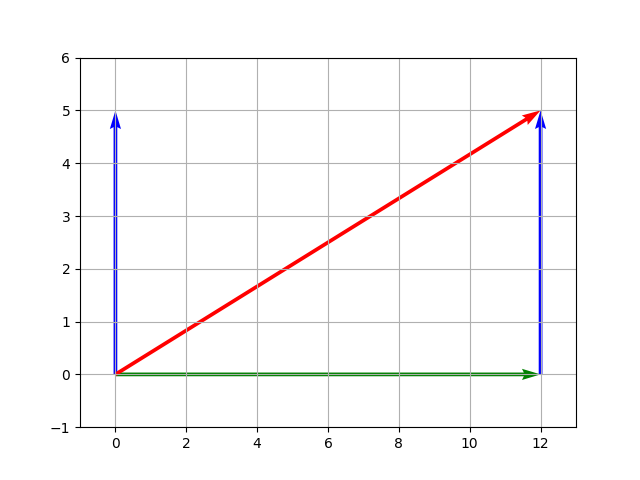
\includegraphics[width=100mm, scale=0.9]{vector_diagram.png}
In the figure, blue arrow with its tail at origin represents $\vec{a}$, which can also be displaced to have its tail at the coordinate (12,0) to complete the triangle.\\
The red arrow represents $\vec{a}+\vec{b}$ (by Triangle Law of Vector Addition) and green arrow represents $\vec{b}$. Vectors $\vec{a}$ and $\vec{b}$ are perpendicular, $\norm{\vec{a}} = 5$ and $\norm{\vec{a}+\vec{b}} = 13$, hence by the diagram, $\norm{\vec{b}}$ should be 12 since by Baudhāyana Sulbasūtra, 5, 12, and 13 form a triplet which is quite famous ($5^2+12^2=13^2$).
\end{document}
